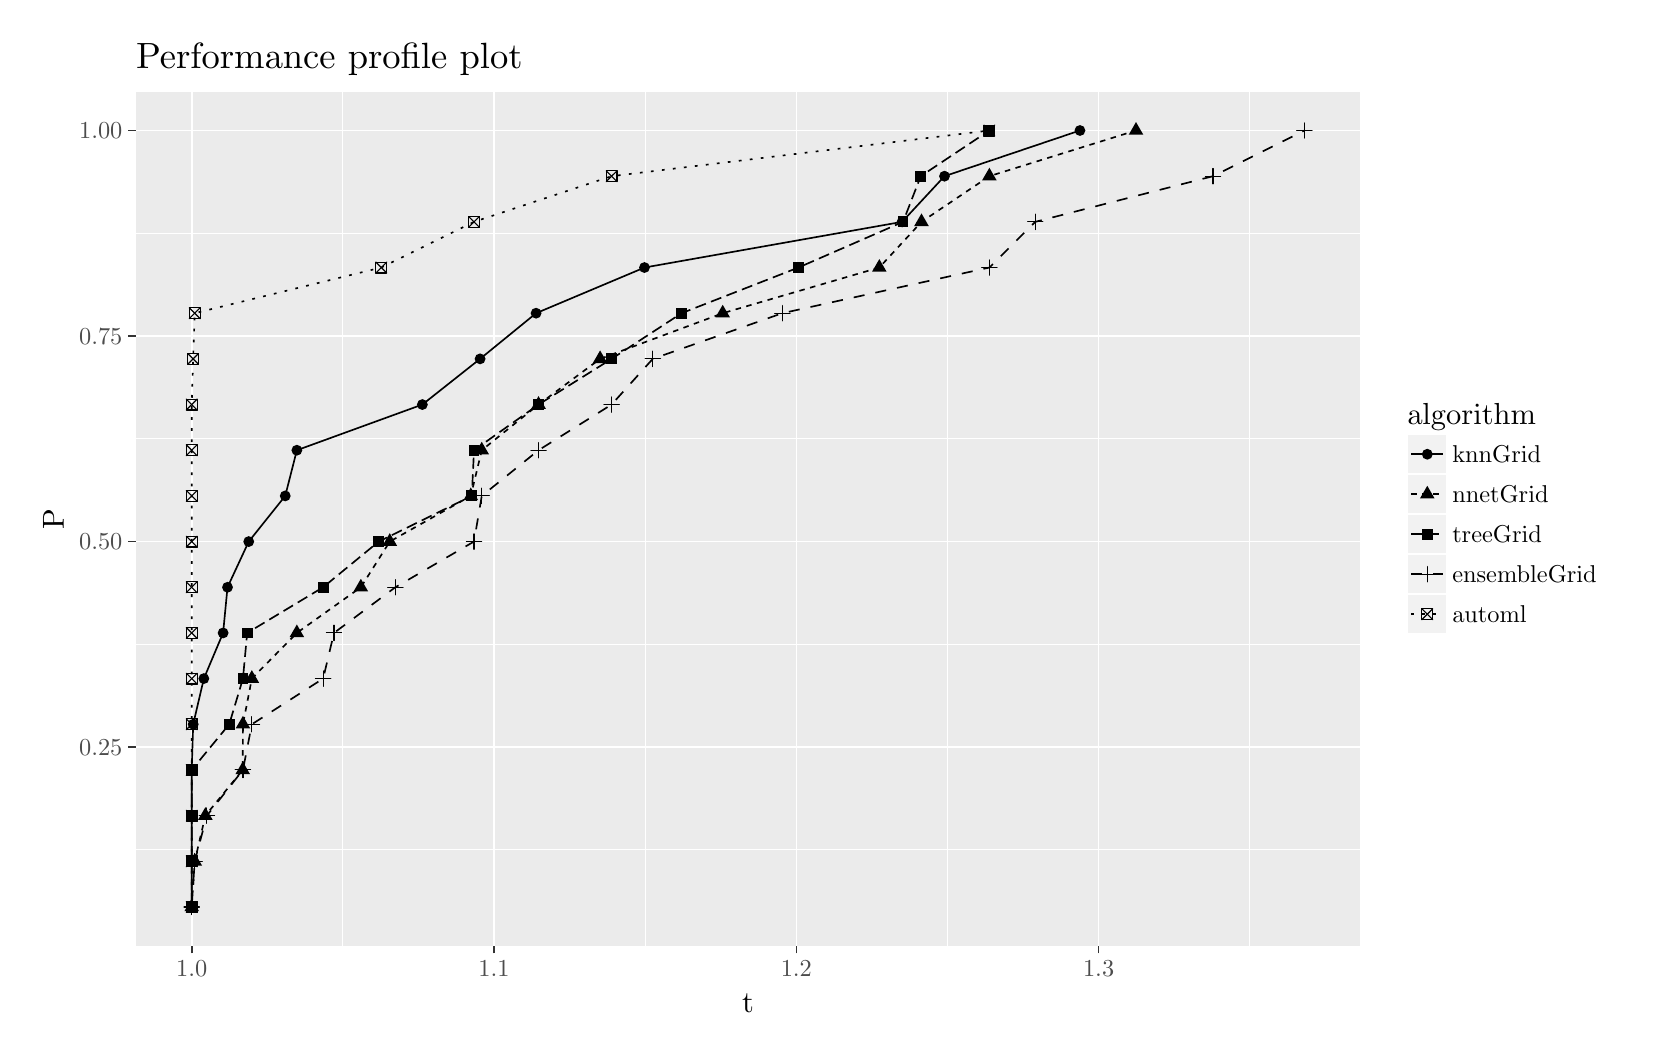
\begin{tikzpicture}[x=1pt,y=1pt]
\definecolor{fillColor}{RGB}{255,255,255}
\path[use as bounding box,fill=fillColor,fill opacity=0.00] (0,0) rectangle (578.16,361.35);
\begin{scope}
\path[clip] (  0.00,  0.00) rectangle (578.16,361.35);
\definecolor{drawColor}{RGB}{255,255,255}
\definecolor{fillColor}{RGB}{255,255,255}

\path[draw=drawColor,line width= 0.6pt,line join=round,line cap=round,fill=fillColor] (  0.00,  0.00) rectangle (578.16,361.35);
\end{scope}
\begin{scope}
\path[clip] ( 39.17, 29.59) rectangle (481.45,338.21);
\definecolor{fillColor}{gray}{0.92}

\path[fill=fillColor] ( 39.17, 29.59) rectangle (481.45,338.21);
\definecolor{drawColor}{RGB}{255,255,255}

\path[draw=drawColor,line width= 0.3pt,line join=round] ( 39.17, 64.25) --
	(481.45, 64.25);

\path[draw=drawColor,line width= 0.3pt,line join=round] ( 39.17,138.51) --
	(481.45,138.51);

\path[draw=drawColor,line width= 0.3pt,line join=round] ( 39.17,212.78) --
	(481.45,212.78);

\path[draw=drawColor,line width= 0.3pt,line join=round] ( 39.17,287.05) --
	(481.45,287.05);

\path[draw=drawColor,line width= 0.3pt,line join=round] (113.89, 29.59) --
	(113.89,338.21);

\path[draw=drawColor,line width= 0.3pt,line join=round] (223.13, 29.59) --
	(223.13,338.21);

\path[draw=drawColor,line width= 0.3pt,line join=round] (332.37, 29.59) --
	(332.37,338.21);

\path[draw=drawColor,line width= 0.3pt,line join=round] (441.61, 29.59) --
	(441.61,338.21);

\path[draw=drawColor,line width= 0.6pt,line join=round] ( 39.17,101.38) --
	(481.45,101.38);

\path[draw=drawColor,line width= 0.6pt,line join=round] ( 39.17,175.65) --
	(481.45,175.65);

\path[draw=drawColor,line width= 0.6pt,line join=round] ( 39.17,249.92) --
	(481.45,249.92);

\path[draw=drawColor,line width= 0.6pt,line join=round] ( 39.17,324.19) --
	(481.45,324.19);

\path[draw=drawColor,line width= 0.6pt,line join=round] ( 59.27, 29.59) --
	( 59.27,338.21);

\path[draw=drawColor,line width= 0.6pt,line join=round] (168.51, 29.59) --
	(168.51,338.21);

\path[draw=drawColor,line width= 0.6pt,line join=round] (277.75, 29.59) --
	(277.75,338.21);

\path[draw=drawColor,line width= 0.6pt,line join=round] (386.99, 29.59) --
	(386.99,338.21);
\definecolor{drawColor}{RGB}{0,0,0}

\path[draw=drawColor,line width= 0.6pt,line join=round] ( 59.27, 43.62) --
	( 59.27, 60.12) --
	( 59.27, 76.62) --
	( 59.27, 93.13) --
	( 59.81,109.63) --
	( 63.66,126.14) --
	( 70.62,142.64) --
	( 72.21,159.14) --
	( 79.88,175.65) --
	( 93.07,192.15) --
	( 97.27,208.66) --
	(142.62,225.16) --
	(163.48,241.67) --
	(183.71,258.17) --
	(222.88,274.67) --
	(315.97,291.18) --
	(331.29,307.68) --
	(380.23,324.19);

\path[draw=drawColor,line width= 0.6pt,dash pattern=on 2pt off 2pt ,line join=round] ( 59.27, 43.62) --
	( 60.36, 60.12) --
	( 64.21, 76.62) --
	( 77.71, 93.13) --
	( 77.79,109.63) --
	( 81.00,126.14) --
	( 97.27,142.64) --
	(120.40,159.14) --
	(130.84,175.65) --
	(160.12,192.15) --
	(164.08,208.66) --
	(184.60,225.16) --
	(206.85,241.67) --
	(251.15,258.17) --
	(307.74,274.67) --
	(322.98,291.18) --
	(347.51,307.68) --
	(400.49,324.19);

\path[draw=drawColor,line width= 0.6pt,dash pattern=on 4pt off 2pt ,line join=round] ( 59.27, 43.62) --
	( 59.27, 60.12) --
	( 59.27, 76.62) --
	( 59.27, 93.13) --
	( 72.83,109.63) --
	( 77.79,126.14) --
	( 79.32,142.64) --
	(106.77,159.14) --
	(126.84,175.65) --
	(160.49,192.15) --
	(161.28,208.66) --
	(184.60,225.16) --
	(211.00,241.67) --
	(236.29,258.17) --
	(278.51,274.67) --
	(316.32,291.18) --
	(322.71,307.68) --
	(347.51,324.19);

\path[draw=drawColor,line width= 0.6pt,dash pattern=on 4pt off 4pt ,line join=round] ( 59.27, 43.62) --
	( 60.36, 60.12) --
	( 64.76, 76.62) --
	( 77.79, 93.13) --
	( 81.00,109.63) --
	(106.77,126.14) --
	(110.69,142.64) --
	(132.86,159.14) --
	(161.28,175.65) --
	(164.08,192.15) --
	(184.60,208.66) --
	(211.00,225.16) --
	(225.88,241.67) --
	(272.69,258.17) --
	(347.51,274.67) --
	(364.08,291.18) --
	(428.32,307.68) --
	(461.34,324.19);

\path[draw=drawColor,line width= 0.6pt,dash pattern=on 1pt off 3pt ,line join=round] ( 59.27, 43.62) --
	( 59.27, 60.12) --
	( 59.27, 76.62) --
	( 59.27, 93.13) --
	( 59.27,109.63) --
	( 59.27,126.14) --
	( 59.27,142.64) --
	( 59.27,159.14) --
	( 59.27,175.65) --
	( 59.27,192.15) --
	( 59.27,208.66) --
	( 59.27,225.16) --
	( 59.79,241.67) --
	( 60.36,258.17) --
	(127.77,274.67) --
	(161.28,291.18) --
	(211.00,307.68) --
	(347.51,324.19);
\definecolor{fillColor}{RGB}{0,0,0}

\path[fill=fillColor] ( 59.27, 43.62) circle (  1.96);

\path[fill=fillColor] ( 59.27, 60.12) circle (  1.96);

\path[fill=fillColor] ( 59.27, 76.62) circle (  1.96);

\path[fill=fillColor] ( 59.27, 93.13) circle (  1.96);

\path[fill=fillColor] ( 59.81,109.63) circle (  1.96);

\path[fill=fillColor] ( 63.66,126.14) circle (  1.96);

\path[fill=fillColor] ( 70.62,142.64) circle (  1.96);

\path[fill=fillColor] ( 72.21,159.14) circle (  1.96);

\path[fill=fillColor] ( 79.88,175.65) circle (  1.96);

\path[fill=fillColor] ( 93.07,192.15) circle (  1.96);

\path[fill=fillColor] ( 97.27,208.66) circle (  1.96);

\path[fill=fillColor] (142.62,225.16) circle (  1.96);

\path[fill=fillColor] (163.48,241.67) circle (  1.96);

\path[fill=fillColor] (183.71,258.17) circle (  1.96);

\path[fill=fillColor] (222.88,274.67) circle (  1.96);

\path[fill=fillColor] (315.97,291.18) circle (  1.96);

\path[fill=fillColor] (331.29,307.68) circle (  1.96);

\path[fill=fillColor] (380.23,324.19) circle (  1.96);

\path[fill=fillColor] ( 59.27, 46.67) --
	( 61.91, 42.09) --
	( 56.63, 42.09) --
	cycle;

\path[fill=fillColor] ( 60.36, 63.17) --
	( 63.00, 58.59) --
	( 57.72, 58.59) --
	cycle;

\path[fill=fillColor] ( 64.21, 79.67) --
	( 66.85, 75.10) --
	( 61.57, 75.10) --
	cycle;

\path[fill=fillColor] ( 77.71, 96.18) --
	( 80.35, 91.60) --
	( 75.07, 91.60) --
	cycle;

\path[fill=fillColor] ( 77.79,112.68) --
	( 80.43,108.11) --
	( 75.14,108.11) --
	cycle;

\path[fill=fillColor] ( 81.00,129.19) --
	( 83.64,124.61) --
	( 78.35,124.61) --
	cycle;

\path[fill=fillColor] ( 97.27,145.69) --
	( 99.91,141.11) --
	( 94.62,141.11) --
	cycle;

\path[fill=fillColor] (120.40,162.20) --
	(123.04,157.62) --
	(117.75,157.62) --
	cycle;

\path[fill=fillColor] (130.84,178.70) --
	(133.49,174.12) --
	(128.20,174.12) --
	cycle;

\path[fill=fillColor] (160.12,195.20) --
	(162.76,190.63) --
	(157.48,190.63) --
	cycle;

\path[fill=fillColor] (164.08,211.71) --
	(166.72,207.13) --
	(161.44,207.13) --
	cycle;

\path[fill=fillColor] (184.60,228.21) --
	(187.24,223.64) --
	(181.96,223.64) --
	cycle;

\path[fill=fillColor] (206.85,244.72) --
	(209.49,240.14) --
	(204.21,240.14) --
	cycle;

\path[fill=fillColor] (251.15,261.22) --
	(253.79,256.64) --
	(248.51,256.64) --
	cycle;

\path[fill=fillColor] (307.74,277.73) --
	(310.38,273.15) --
	(305.10,273.15) --
	cycle;

\path[fill=fillColor] (322.98,294.23) --
	(325.62,289.65) --
	(320.33,289.65) --
	cycle;

\path[fill=fillColor] (347.51,310.73) --
	(350.15,306.16) --
	(344.86,306.16) --
	cycle;

\path[fill=fillColor] (400.49,327.24) --
	(403.14,322.66) --
	(397.85,322.66) --
	cycle;

\path[fill=fillColor] ( 57.31, 41.65) --
	( 61.23, 41.65) --
	( 61.23, 45.58) --
	( 57.31, 45.58) --
	cycle;

\path[fill=fillColor] ( 57.31, 58.16) --
	( 61.23, 58.16) --
	( 61.23, 62.08) --
	( 57.31, 62.08) --
	cycle;

\path[fill=fillColor] ( 57.31, 74.66) --
	( 61.23, 74.66) --
	( 61.23, 78.59) --
	( 57.31, 78.59) --
	cycle;

\path[fill=fillColor] ( 57.31, 91.17) --
	( 61.23, 91.17) --
	( 61.23, 95.09) --
	( 57.31, 95.09) --
	cycle;

\path[fill=fillColor] ( 70.87,107.67) --
	( 74.79,107.67) --
	( 74.79,111.59) --
	( 70.87,111.59) --
	cycle;

\path[fill=fillColor] ( 75.82,124.17) --
	( 79.75,124.17) --
	( 79.75,128.10) --
	( 75.82,128.10) --
	cycle;

\path[fill=fillColor] ( 77.36,140.68) --
	( 81.29,140.68) --
	( 81.29,144.60) --
	( 77.36,144.60) --
	cycle;

\path[fill=fillColor] (104.80,157.18) --
	(108.73,157.18) --
	(108.73,161.11) --
	(104.80,161.11) --
	cycle;

\path[fill=fillColor] (124.87,173.69) --
	(128.80,173.69) --
	(128.80,177.61) --
	(124.87,177.61) --
	cycle;

\path[fill=fillColor] (158.53,190.19) --
	(162.45,190.19) --
	(162.45,194.12) --
	(158.53,194.12) --
	cycle;

\path[fill=fillColor] (159.32,206.69) --
	(163.24,206.69) --
	(163.24,210.62) --
	(159.32,210.62) --
	cycle;

\path[fill=fillColor] (182.64,223.20) --
	(186.56,223.20) --
	(186.56,227.12) --
	(182.64,227.12) --
	cycle;

\path[fill=fillColor] (209.03,239.70) --
	(212.96,239.70) --
	(212.96,243.63) --
	(209.03,243.63) --
	cycle;

\path[fill=fillColor] (234.33,256.21) --
	(238.25,256.21) --
	(238.25,260.13) --
	(234.33,260.13) --
	cycle;

\path[fill=fillColor] (276.54,272.71) --
	(280.47,272.71) --
	(280.47,276.64) --
	(276.54,276.64) --
	cycle;

\path[fill=fillColor] (314.36,289.22) --
	(318.28,289.22) --
	(318.28,293.14) --
	(314.36,293.14) --
	cycle;

\path[fill=fillColor] (320.75,305.72) --
	(324.67,305.72) --
	(324.67,309.64) --
	(320.75,309.64) --
	cycle;

\path[fill=fillColor] (345.54,322.22) --
	(349.47,322.22) --
	(349.47,326.15) --
	(345.54,326.15) --
	cycle;

\path[draw=drawColor,line width= 0.4pt,line join=round,line cap=round] ( 56.50, 43.62) -- ( 62.05, 43.62);

\path[draw=drawColor,line width= 0.4pt,line join=round,line cap=round] ( 59.27, 40.84) -- ( 59.27, 46.39);

\path[draw=drawColor,line width= 0.4pt,line join=round,line cap=round] ( 57.59, 60.12) -- ( 63.14, 60.12);

\path[draw=drawColor,line width= 0.4pt,line join=round,line cap=round] ( 60.36, 57.34) -- ( 60.36, 62.89);

\path[draw=drawColor,line width= 0.4pt,line join=round,line cap=round] ( 61.98, 76.62) -- ( 67.53, 76.62);

\path[draw=drawColor,line width= 0.4pt,line join=round,line cap=round] ( 64.76, 73.85) -- ( 64.76, 79.40);

\path[draw=drawColor,line width= 0.4pt,line join=round,line cap=round] ( 75.01, 93.13) -- ( 80.56, 93.13);

\path[draw=drawColor,line width= 0.4pt,line join=round,line cap=round] ( 77.79, 90.35) -- ( 77.79, 95.90);

\path[draw=drawColor,line width= 0.4pt,line join=round,line cap=round] ( 78.22,109.63) -- ( 83.77,109.63);

\path[draw=drawColor,line width= 0.4pt,line join=round,line cap=round] ( 81.00,106.86) -- ( 81.00,112.41);

\path[draw=drawColor,line width= 0.4pt,line join=round,line cap=round] (103.99,126.14) -- (109.54,126.14);

\path[draw=drawColor,line width= 0.4pt,line join=round,line cap=round] (106.77,123.36) -- (106.77,128.91);

\path[draw=drawColor,line width= 0.4pt,line join=round,line cap=round] (107.91,142.64) -- (113.46,142.64);

\path[draw=drawColor,line width= 0.4pt,line join=round,line cap=round] (110.69,139.87) -- (110.69,145.42);

\path[draw=drawColor,line width= 0.4pt,line join=round,line cap=round] (130.09,159.14) -- (135.64,159.14);

\path[draw=drawColor,line width= 0.4pt,line join=round,line cap=round] (132.86,156.37) -- (132.86,161.92);

\path[draw=drawColor,line width= 0.4pt,line join=round,line cap=round] (158.51,175.65) -- (164.06,175.65);

\path[draw=drawColor,line width= 0.4pt,line join=round,line cap=round] (161.28,172.87) -- (161.28,178.42);

\path[draw=drawColor,line width= 0.4pt,line join=round,line cap=round] (161.30,192.15) -- (166.85,192.15);

\path[draw=drawColor,line width= 0.4pt,line join=round,line cap=round] (164.08,189.38) -- (164.08,194.93);

\path[draw=drawColor,line width= 0.4pt,line join=round,line cap=round] (181.82,208.66) -- (187.37,208.66);

\path[draw=drawColor,line width= 0.4pt,line join=round,line cap=round] (184.60,205.88) -- (184.60,211.43);

\path[draw=drawColor,line width= 0.4pt,line join=round,line cap=round] (208.22,225.16) -- (213.77,225.16);

\path[draw=drawColor,line width= 0.4pt,line join=round,line cap=round] (211.00,222.39) -- (211.00,227.94);

\path[draw=drawColor,line width= 0.4pt,line join=round,line cap=round] (223.11,241.67) -- (228.66,241.67);

\path[draw=drawColor,line width= 0.4pt,line join=round,line cap=round] (225.88,238.89) -- (225.88,244.44);

\path[draw=drawColor,line width= 0.4pt,line join=round,line cap=round] (269.92,258.17) -- (275.47,258.17);

\path[draw=drawColor,line width= 0.4pt,line join=round,line cap=round] (272.69,255.39) -- (272.69,260.94);

\path[draw=drawColor,line width= 0.4pt,line join=round,line cap=round] (344.73,274.67) -- (350.28,274.67);

\path[draw=drawColor,line width= 0.4pt,line join=round,line cap=round] (347.51,271.90) -- (347.51,277.45);

\path[draw=drawColor,line width= 0.4pt,line join=round,line cap=round] (361.31,291.18) -- (366.86,291.18);

\path[draw=drawColor,line width= 0.4pt,line join=round,line cap=round] (364.08,288.40) -- (364.08,293.95);

\path[draw=drawColor,line width= 0.4pt,line join=round,line cap=round] (425.55,307.68) -- (431.09,307.68);

\path[draw=drawColor,line width= 0.4pt,line join=round,line cap=round] (428.32,304.91) -- (428.32,310.46);

\path[draw=drawColor,line width= 0.4pt,line join=round,line cap=round] (458.57,324.19) -- (464.12,324.19);

\path[draw=drawColor,line width= 0.4pt,line join=round,line cap=round] (461.34,321.41) -- (461.34,326.96);

\path[draw=drawColor,line width= 0.4pt,line join=round,line cap=round] ( 57.31, 41.65) rectangle ( 61.23, 45.58);

\path[draw=drawColor,line width= 0.4pt,line join=round,line cap=round] ( 57.31, 41.65) -- ( 61.23, 45.58);

\path[draw=drawColor,line width= 0.4pt,line join=round,line cap=round] ( 57.31, 45.58) -- ( 61.23, 41.65);

\path[draw=drawColor,line width= 0.4pt,line join=round,line cap=round] ( 57.31, 58.16) rectangle ( 61.23, 62.08);

\path[draw=drawColor,line width= 0.4pt,line join=round,line cap=round] ( 57.31, 58.16) -- ( 61.23, 62.08);

\path[draw=drawColor,line width= 0.4pt,line join=round,line cap=round] ( 57.31, 62.08) -- ( 61.23, 58.16);

\path[draw=drawColor,line width= 0.4pt,line join=round,line cap=round] ( 57.31, 74.66) rectangle ( 61.23, 78.59);

\path[draw=drawColor,line width= 0.4pt,line join=round,line cap=round] ( 57.31, 74.66) -- ( 61.23, 78.59);

\path[draw=drawColor,line width= 0.4pt,line join=round,line cap=round] ( 57.31, 78.59) -- ( 61.23, 74.66);

\path[draw=drawColor,line width= 0.4pt,line join=round,line cap=round] ( 57.31, 91.17) rectangle ( 61.23, 95.09);

\path[draw=drawColor,line width= 0.4pt,line join=round,line cap=round] ( 57.31, 91.17) -- ( 61.23, 95.09);

\path[draw=drawColor,line width= 0.4pt,line join=round,line cap=round] ( 57.31, 95.09) -- ( 61.23, 91.17);

\path[draw=drawColor,line width= 0.4pt,line join=round,line cap=round] ( 57.31,107.67) rectangle ( 61.23,111.59);

\path[draw=drawColor,line width= 0.4pt,line join=round,line cap=round] ( 57.31,107.67) -- ( 61.23,111.59);

\path[draw=drawColor,line width= 0.4pt,line join=round,line cap=round] ( 57.31,111.59) -- ( 61.23,107.67);

\path[draw=drawColor,line width= 0.4pt,line join=round,line cap=round] ( 57.31,124.17) rectangle ( 61.23,128.10);

\path[draw=drawColor,line width= 0.4pt,line join=round,line cap=round] ( 57.31,124.17) -- ( 61.23,128.10);

\path[draw=drawColor,line width= 0.4pt,line join=round,line cap=round] ( 57.31,128.10) -- ( 61.23,124.17);

\path[draw=drawColor,line width= 0.4pt,line join=round,line cap=round] ( 57.31,140.68) rectangle ( 61.23,144.60);

\path[draw=drawColor,line width= 0.4pt,line join=round,line cap=round] ( 57.31,140.68) -- ( 61.23,144.60);

\path[draw=drawColor,line width= 0.4pt,line join=round,line cap=round] ( 57.31,144.60) -- ( 61.23,140.68);

\path[draw=drawColor,line width= 0.4pt,line join=round,line cap=round] ( 57.31,157.18) rectangle ( 61.23,161.11);

\path[draw=drawColor,line width= 0.4pt,line join=round,line cap=round] ( 57.31,157.18) -- ( 61.23,161.11);

\path[draw=drawColor,line width= 0.4pt,line join=round,line cap=round] ( 57.31,161.11) -- ( 61.23,157.18);

\path[draw=drawColor,line width= 0.4pt,line join=round,line cap=round] ( 57.31,173.69) rectangle ( 61.23,177.61);

\path[draw=drawColor,line width= 0.4pt,line join=round,line cap=round] ( 57.31,173.69) -- ( 61.23,177.61);

\path[draw=drawColor,line width= 0.4pt,line join=round,line cap=round] ( 57.31,177.61) -- ( 61.23,173.69);

\path[draw=drawColor,line width= 0.4pt,line join=round,line cap=round] ( 57.31,190.19) rectangle ( 61.23,194.12);

\path[draw=drawColor,line width= 0.4pt,line join=round,line cap=round] ( 57.31,190.19) -- ( 61.23,194.12);

\path[draw=drawColor,line width= 0.4pt,line join=round,line cap=round] ( 57.31,194.12) -- ( 61.23,190.19);

\path[draw=drawColor,line width= 0.4pt,line join=round,line cap=round] ( 57.31,206.69) rectangle ( 61.23,210.62);

\path[draw=drawColor,line width= 0.4pt,line join=round,line cap=round] ( 57.31,206.69) -- ( 61.23,210.62);

\path[draw=drawColor,line width= 0.4pt,line join=round,line cap=round] ( 57.31,210.62) -- ( 61.23,206.69);

\path[draw=drawColor,line width= 0.4pt,line join=round,line cap=round] ( 57.31,223.20) rectangle ( 61.23,227.12);

\path[draw=drawColor,line width= 0.4pt,line join=round,line cap=round] ( 57.31,223.20) -- ( 61.23,227.12);

\path[draw=drawColor,line width= 0.4pt,line join=round,line cap=round] ( 57.31,227.12) -- ( 61.23,223.20);

\path[draw=drawColor,line width= 0.4pt,line join=round,line cap=round] ( 57.83,239.70) rectangle ( 61.75,243.63);

\path[draw=drawColor,line width= 0.4pt,line join=round,line cap=round] ( 57.83,239.70) -- ( 61.75,243.63);

\path[draw=drawColor,line width= 0.4pt,line join=round,line cap=round] ( 57.83,243.63) -- ( 61.75,239.70);

\path[draw=drawColor,line width= 0.4pt,line join=round,line cap=round] ( 58.40,256.21) rectangle ( 62.32,260.13);

\path[draw=drawColor,line width= 0.4pt,line join=round,line cap=round] ( 58.40,256.21) -- ( 62.32,260.13);

\path[draw=drawColor,line width= 0.4pt,line join=round,line cap=round] ( 58.40,260.13) -- ( 62.32,256.21);

\path[draw=drawColor,line width= 0.4pt,line join=round,line cap=round] (125.81,272.71) rectangle (129.73,276.64);

\path[draw=drawColor,line width= 0.4pt,line join=round,line cap=round] (125.81,272.71) -- (129.73,276.64);

\path[draw=drawColor,line width= 0.4pt,line join=round,line cap=round] (125.81,276.64) -- (129.73,272.71);

\path[draw=drawColor,line width= 0.4pt,line join=round,line cap=round] (159.32,289.22) rectangle (163.24,293.14);

\path[draw=drawColor,line width= 0.4pt,line join=round,line cap=round] (159.32,289.22) -- (163.24,293.14);

\path[draw=drawColor,line width= 0.4pt,line join=round,line cap=round] (159.32,293.14) -- (163.24,289.22);

\path[draw=drawColor,line width= 0.4pt,line join=round,line cap=round] (209.03,305.72) rectangle (212.96,309.64);

\path[draw=drawColor,line width= 0.4pt,line join=round,line cap=round] (209.03,305.72) -- (212.96,309.64);

\path[draw=drawColor,line width= 0.4pt,line join=round,line cap=round] (209.03,309.64) -- (212.96,305.72);

\path[draw=drawColor,line width= 0.4pt,line join=round,line cap=round] (345.54,322.22) rectangle (349.47,326.15);

\path[draw=drawColor,line width= 0.4pt,line join=round,line cap=round] (345.54,322.22) -- (349.47,326.15);

\path[draw=drawColor,line width= 0.4pt,line join=round,line cap=round] (345.54,326.15) -- (349.47,322.22);
\end{scope}
\begin{scope}
\path[clip] (  0.00,  0.00) rectangle (578.16,361.35);
\definecolor{drawColor}{gray}{0.30}

\node[text=drawColor,anchor=base east,inner sep=0pt, outer sep=0pt, scale=  0.88] at ( 34.22, 98.35) {0.25};

\node[text=drawColor,anchor=base east,inner sep=0pt, outer sep=0pt, scale=  0.88] at ( 34.22,172.62) {0.50};

\node[text=drawColor,anchor=base east,inner sep=0pt, outer sep=0pt, scale=  0.88] at ( 34.22,246.89) {0.75};

\node[text=drawColor,anchor=base east,inner sep=0pt, outer sep=0pt, scale=  0.88] at ( 34.22,321.16) {1.00};
\end{scope}
\begin{scope}
\path[clip] (  0.00,  0.00) rectangle (578.16,361.35);
\definecolor{drawColor}{gray}{0.20}

\path[draw=drawColor,line width= 0.6pt,line join=round] ( 36.42,101.38) --
	( 39.17,101.38);

\path[draw=drawColor,line width= 0.6pt,line join=round] ( 36.42,175.65) --
	( 39.17,175.65);

\path[draw=drawColor,line width= 0.6pt,line join=round] ( 36.42,249.92) --
	( 39.17,249.92);

\path[draw=drawColor,line width= 0.6pt,line join=round] ( 36.42,324.19) --
	( 39.17,324.19);
\end{scope}
\begin{scope}
\path[clip] (  0.00,  0.00) rectangle (578.16,361.35);
\definecolor{drawColor}{gray}{0.20}

\path[draw=drawColor,line width= 0.6pt,line join=round] ( 59.27, 26.84) --
	( 59.27, 29.59);

\path[draw=drawColor,line width= 0.6pt,line join=round] (168.51, 26.84) --
	(168.51, 29.59);

\path[draw=drawColor,line width= 0.6pt,line join=round] (277.75, 26.84) --
	(277.75, 29.59);

\path[draw=drawColor,line width= 0.6pt,line join=round] (386.99, 26.84) --
	(386.99, 29.59);
\end{scope}
\begin{scope}
\path[clip] (  0.00,  0.00) rectangle (578.16,361.35);
\definecolor{drawColor}{gray}{0.30}

\node[text=drawColor,anchor=base,inner sep=0pt, outer sep=0pt, scale=  0.88] at ( 59.27, 18.58) {1.0};

\node[text=drawColor,anchor=base,inner sep=0pt, outer sep=0pt, scale=  0.88] at (168.51, 18.58) {1.1};

\node[text=drawColor,anchor=base,inner sep=0pt, outer sep=0pt, scale=  0.88] at (277.75, 18.58) {1.2};

\node[text=drawColor,anchor=base,inner sep=0pt, outer sep=0pt, scale=  0.88] at (386.99, 18.58) {1.3};
\end{scope}
\begin{scope}
\path[clip] (  0.00,  0.00) rectangle (578.16,361.35);
\definecolor{drawColor}{RGB}{0,0,0}

\node[text=drawColor,anchor=base,inner sep=0pt, outer sep=0pt, scale=  1.10] at (260.31,  5.50) {t};
\end{scope}
\begin{scope}
\path[clip] (  0.00,  0.00) rectangle (578.16,361.35);
\definecolor{drawColor}{RGB}{0,0,0}

\node[text=drawColor,rotate= 90.00,anchor=base,inner sep=0pt, outer sep=0pt, scale=  1.10] at ( 13.08,183.90) {P};
\end{scope}
\begin{scope}
\path[clip] (  0.00,  0.00) rectangle (578.16,361.35);
\definecolor{fillColor}{RGB}{255,255,255}

\path[fill=fillColor] (492.83,136.48) rectangle (572.66,231.32);
\end{scope}
\begin{scope}
\path[clip] (  0.00,  0.00) rectangle (578.16,361.35);
\definecolor{drawColor}{RGB}{0,0,0}

\node[text=drawColor,anchor=base west,inner sep=0pt, outer sep=0pt, scale=  1.10] at (498.52,218.05) {algorithm};
\end{scope}
\begin{scope}
\path[clip] (  0.00,  0.00) rectangle (578.16,361.35);
\definecolor{drawColor}{RGB}{255,255,255}
\definecolor{fillColor}{gray}{0.95}

\path[draw=drawColor,line width= 0.6pt,line join=round,line cap=round,fill=fillColor] (498.52,199.99) rectangle (512.97,214.44);
\end{scope}
\begin{scope}
\path[clip] (  0.00,  0.00) rectangle (578.16,361.35);
\definecolor{drawColor}{RGB}{0,0,0}

\path[draw=drawColor,line width= 0.6pt,line join=round] (499.97,207.21) -- (511.53,207.21);
\end{scope}
\begin{scope}
\path[clip] (  0.00,  0.00) rectangle (578.16,361.35);
\definecolor{fillColor}{RGB}{0,0,0}

\path[fill=fillColor] (505.75,207.21) circle (  1.96);
\end{scope}
\begin{scope}
\path[clip] (  0.00,  0.00) rectangle (578.16,361.35);
\definecolor{drawColor}{RGB}{255,255,255}
\definecolor{fillColor}{gray}{0.95}

\path[draw=drawColor,line width= 0.6pt,line join=round,line cap=round,fill=fillColor] (498.52,185.53) rectangle (512.97,199.99);
\end{scope}
\begin{scope}
\path[clip] (  0.00,  0.00) rectangle (578.16,361.35);
\definecolor{drawColor}{RGB}{0,0,0}

\path[draw=drawColor,line width= 0.6pt,dash pattern=on 2pt off 2pt ,line join=round] (499.97,192.76) -- (511.53,192.76);
\end{scope}
\begin{scope}
\path[clip] (  0.00,  0.00) rectangle (578.16,361.35);
\definecolor{fillColor}{RGB}{0,0,0}

\path[fill=fillColor] (505.75,195.81) --
	(508.39,191.23) --
	(503.10,191.23) --
	cycle;
\end{scope}
\begin{scope}
\path[clip] (  0.00,  0.00) rectangle (578.16,361.35);
\definecolor{drawColor}{RGB}{255,255,255}
\definecolor{fillColor}{gray}{0.95}

\path[draw=drawColor,line width= 0.6pt,line join=round,line cap=round,fill=fillColor] (498.52,171.08) rectangle (512.97,185.53);
\end{scope}
\begin{scope}
\path[clip] (  0.00,  0.00) rectangle (578.16,361.35);
\definecolor{drawColor}{RGB}{0,0,0}

\path[draw=drawColor,line width= 0.6pt,dash pattern=on 4pt off 2pt ,line join=round] (499.97,178.31) -- (511.53,178.31);
\end{scope}
\begin{scope}
\path[clip] (  0.00,  0.00) rectangle (578.16,361.35);
\definecolor{fillColor}{RGB}{0,0,0}

\path[fill=fillColor] (503.78,176.34) --
	(507.71,176.34) --
	(507.71,180.27) --
	(503.78,180.27) --
	cycle;
\end{scope}
\begin{scope}
\path[clip] (  0.00,  0.00) rectangle (578.16,361.35);
\definecolor{drawColor}{RGB}{255,255,255}
\definecolor{fillColor}{gray}{0.95}

\path[draw=drawColor,line width= 0.6pt,line join=round,line cap=round,fill=fillColor] (498.52,156.63) rectangle (512.97,171.08);
\end{scope}
\begin{scope}
\path[clip] (  0.00,  0.00) rectangle (578.16,361.35);
\definecolor{drawColor}{RGB}{0,0,0}

\path[draw=drawColor,line width= 0.6pt,dash pattern=on 4pt off 4pt ,line join=round] (499.97,163.85) -- (511.53,163.85);
\end{scope}
\begin{scope}
\path[clip] (  0.00,  0.00) rectangle (578.16,361.35);
\definecolor{drawColor}{RGB}{0,0,0}

\path[draw=drawColor,line width= 0.4pt,line join=round,line cap=round] (502.97,163.85) -- (508.52,163.85);

\path[draw=drawColor,line width= 0.4pt,line join=round,line cap=round] (505.75,161.08) -- (505.75,166.63);
\end{scope}
\begin{scope}
\path[clip] (  0.00,  0.00) rectangle (578.16,361.35);
\definecolor{drawColor}{RGB}{255,255,255}
\definecolor{fillColor}{gray}{0.95}

\path[draw=drawColor,line width= 0.6pt,line join=round,line cap=round,fill=fillColor] (498.52,142.17) rectangle (512.97,156.63);
\end{scope}
\begin{scope}
\path[clip] (  0.00,  0.00) rectangle (578.16,361.35);
\definecolor{drawColor}{RGB}{0,0,0}

\path[draw=drawColor,line width= 0.6pt,dash pattern=on 1pt off 3pt ,line join=round] (499.97,149.40) -- (511.53,149.40);
\end{scope}
\begin{scope}
\path[clip] (  0.00,  0.00) rectangle (578.16,361.35);
\definecolor{drawColor}{RGB}{0,0,0}

\path[draw=drawColor,line width= 0.4pt,line join=round,line cap=round] (503.78,147.44) rectangle (507.71,151.36);

\path[draw=drawColor,line width= 0.4pt,line join=round,line cap=round] (503.78,147.44) -- (507.71,151.36);

\path[draw=drawColor,line width= 0.4pt,line join=round,line cap=round] (503.78,151.36) -- (507.71,147.44);
\end{scope}
\begin{scope}
\path[clip] (  0.00,  0.00) rectangle (578.16,361.35);
\definecolor{drawColor}{RGB}{0,0,0}

\node[text=drawColor,anchor=base west,inner sep=0pt, outer sep=0pt, scale=  0.88] at (514.78,204.18) {knnGrid};
\end{scope}
\begin{scope}
\path[clip] (  0.00,  0.00) rectangle (578.16,361.35);
\definecolor{drawColor}{RGB}{0,0,0}

\node[text=drawColor,anchor=base west,inner sep=0pt, outer sep=0pt, scale=  0.88] at (514.78,189.73) {nnetGrid};
\end{scope}
\begin{scope}
\path[clip] (  0.00,  0.00) rectangle (578.16,361.35);
\definecolor{drawColor}{RGB}{0,0,0}

\node[text=drawColor,anchor=base west,inner sep=0pt, outer sep=0pt, scale=  0.88] at (514.78,175.28) {treeGrid};
\end{scope}
\begin{scope}
\path[clip] (  0.00,  0.00) rectangle (578.16,361.35);
\definecolor{drawColor}{RGB}{0,0,0}

\node[text=drawColor,anchor=base west,inner sep=0pt, outer sep=0pt, scale=  0.88] at (514.78,160.82) {ensembleGrid};
\end{scope}
\begin{scope}
\path[clip] (  0.00,  0.00) rectangle (578.16,361.35);
\definecolor{drawColor}{RGB}{0,0,0}

\node[text=drawColor,anchor=base west,inner sep=0pt, outer sep=0pt, scale=  0.88] at (514.78,146.37) {automl};
\end{scope}
\begin{scope}
\path[clip] (  0.00,  0.00) rectangle (578.16,361.35);
\definecolor{drawColor}{RGB}{0,0,0}

\node[text=drawColor,anchor=base west,inner sep=0pt, outer sep=0pt, scale=  1.32] at ( 39.17,346.76) {Performance profile plot};
\end{scope}
\end{tikzpicture}

